\chapter{Homotopía}%
\label{cha:homotopia}
\section{Conceptos fundamentales}%
\label{sec:conceptos_fundamentales}
\begin{defi}
Una \textbf{homotopía} es una aplicación continua $H : Y \times \left[ 0, 1 \right] \rightarrow X$.
\end{defi}
\begin{obs}
\begin{enumerate}
    \item $H_s : Y \rightarrow X: y \mapsto H\left( y, s \right),\ H \equiv \{H_s: 0 \le s \le 1\}$ familia uniparamétrica de aplicaciones.
    \item Siendo $f = H_0$ y $g = H_1$:
    \[
    \begin{cases}
        H_s : f \simeq g \text{, homotopía entre } f \text{ y } g\\
        H \text{ deformación continua de } f \text{ a } g
    \end{cases} 
    \]
    Con esto, el problema que deseamos resolver es ver cuándo dos aplicaciones son \textbf{homótopas}:
    \[
    \boxed{f \simeq g} 
    \]

    \item $f \simeq g$ relación de equivalencia:
    \begin{itemize}
        \item $f \simeq f$ vía $H_s \equiv f$.
        \item $H_s : f \simeq g \Rightarrow H_{1 - s} : g \simeq f$.
        \item $\begin{rcases}
            F_s : f \simeq g\\
            G_s: g \simeq h
        \end{rcases} \Rightarrow H_s = \begin{cases}
            F_{2s},\ 0 \le s \le 1/2\\
            G_{2s - 1}\ 1/2 \le s \le 1
        \end{cases}: f \simeq h$
        \begin{demo}
            Continuidad: $\begin{cases}
            F_{2(1/2)} = F_1 = g\\
            G_{2(1/2) - 1} = G_0 = g
            \end{cases}$. En el resto de puntos la continuidad se da por serlo $F$ y $G$.
        \end{demo}
        Como notación tenemos que $H_s = F_s * H_s$.
    \end{itemize}
\end{enumerate}

Habitualmente tomamos como hipótesis que el espacio sea conexo por caminos y conexo local por caminos.
\end{obs}

\begin{prop}
$X$ conexo por caminos, $f, g: Y \rightarrow X$ constantes $\Rightarrow f \simeq g$.
\end{prop}
\begin{demo}
Por hipótesis tenemos que $f \equiv x_0$ y $g \equiv x_1$. Entonces, como $\exists \sigma: \left[ 0, 1 \right] \rightarrow X,\ \sigma\left( 0 \right) = x_0$ y $\sigma\left( 1 \right) = x_1 \Rightarrow H_s \equiv \sigma\left( s \right) : \begin{cases}
    H_0 \equiv \sigma\left( 0 \right) = x_0 \equiv f\\
    H_1 \equiv \sigma\left( 1 \right) = x_1 \equiv g
\end{cases}$
\end{demo}

\begin{defi}
$f: Y \rightarrow X$ es \textbf{nulhomótopa} si $f \simeq $ constante, \textbf{esencial} en caso contrario.
\end{defi}

\begin{theo}[Problema esencial. Fibración de Hopf]
(1932) $\exists f : \mathbb{S}^3 \rightarrow \mathbb{S}^2$ esencial con $\mathbb{S}^3 \subset \mathbb{R}^4 = \mathbb{C}^2$ y $\mathbb{S}^2 \subset \mathbb{R}^3 = \mathbb{R} \times \mathbb{C}$:
\[
\left( z, z' \right) \mapsto \left( \lVert z \rVert^2 - \lVert z' \rVert^2, 2 z z'\right)
\]
\end{theo}
Este ejemplo es importante porque demuestra que no todas las aplicaciones son nulhomótopas.

\section{Concepto relativo}%
\label{sec:concepto_relativo}
\begin{defi}
$H: Y \times \left[ 0, 1 \right] \rightarrow X$ es una \textbf{homotopía relativa a} $A \subset Y$ si $H_s\left( a \right) = H_0\left( a \right),\ \forall a \in A$ y $\forall s \in \left[ 0, 1 \right]$.
\end{defi}

\begin{prop}
$H$ relativa a $A,\ f = H_0,\ g = H_1 \Rightarrow f|_A = g|_A$. Notación: $H_s = f \stackrel{A}{\simeq} g$ (Relación de equivalencia).
\end{prop}

\begin{ej}[Fundamentales. Interpolación]
\begin{enumerate}
    \item $f, g: Y \rightarrow X \subset \mathbb{R}^n$ convexo $\Rightarrow\exists H_s = \left( 1 - s \right) f + sg: f \simeq g$.
    \begin{demo}
        Pues por convexidad $H_s\left( y \right) \in \underbrace{\left[ f\left( y \right), g\left( y \right) \right] \subset X}_{\text{\textbf{cond. crucial!}}}$.
    \end{demo}
    $f\left( a \right) = g\left( a \right) \Rightarrow H_s\left( a \right) = \left( 1 - s \right)f\left( a \right) + sg\left( a \right) = f\left( a \right) = g\left( a \right) \Rightarrow H_s$ es relativa a $A = \{f = g\}$.

    Con esto vemos que dos funciones continuas en un convexo con homótopas.

    \item $f: Y \rightarrow X \subset \mathbb{R}^n$ estrellado respecto de $x_0,\ \left[ x, x_0 \right] \subset X,\ \forall x \in X \Rightarrow H_s = \left( 1 - s \right)f + sx_0: f \simeq x_0$ (relativa a $A = f^{-1}\left( x_0 \right)$).

    De nuevo, por transitividad, dos funciones continuas en un estrellado son homótopas.

    \item Variante en $\mathbb{S}^n$:
    %TODO: Imagen
    \begin{center}
        \includegraphics[scale=0.3]{images/ej_fund_interp_3} 
    \end{center}
\end{enumerate} 
\end{ej}

\section{Contractibilidad}%
\label{sec:contractibilidad}
\begin{defi}
$X$ es \textbf{contráctil} si $id: X \rightarrow X$ es nulhomótopa: $\exists H_s : id \simeq x_0$.

Y \textbf{fuertemente contrátil} si $\exists H_s : id \stackrel{x_0}{\simeq} x_0$ (homótopa relativa a $\{x_0\}$)
\end{defi}

\begin{obs}
Los ejemplos son difíciles, pero son cosas distintas.
\end{obs}

\begin{ej}
    $X \subset \mathbb{R}^n$ estrellado respecto $x_0 \Rightarrow$ fuertemente contráctil
    \begin{demo}
        $H_s = \left( 1 - s \right) id + sx_0$.
    \end{demo}
\end{ej}

\begin{prop}
\begin{enumerate}
    \item Si $X$ es contrátil $\Rightarrow$ es conexo por caminos.
    \item Si $X$ es contráctil $\Rightarrow \begin{cases}
        \forall f: Y \rightarrow X \text{ nulhomótopa.}\\
        \forall g: X \rightarrow Z \text{ nulhomótopa.} 
    \end{cases} $
\end{enumerate}
\end{prop}
\begin{demo}
\begin{enumerate}
    \item $H_s: id \simeq x_0 \Rightarrow S \mapsto H_s\left( x_0 \right)$ camino de $x$ a $x_0$.
    \item $H_s: id \simeq x_0 \begin{cases}
        H_s \circ f: f \simeq x_0\\
        g \circ H_s: g \simeq g\left( x_0 \right) 
    \end{cases} $
\end{enumerate}
\end{demo}
\begin{obs}
Pocos espacios son contráctiles, pero no es inmediato verlo.
\end{obs}


\chapter{Homotopía de caminos}%
\label{cha:homotopia_de_caminos}
\section{El concepto básico}%
\label{sec:el_concepto_basico}
\begin{defi}
Sean $\sigma, \tau: \left[ a, b \right] \rightarrow X$, decimos que son homótopos \textbf{con extremos fijos} si $\exists H_s: \sigma \simeq \tau$ relativa a $\{a, b\}$: 
\[
\begin{cases}
    H_s\left( a \right) = \sigma\left( a \right) = \tau\left( a \right)\\
    H_s\left( b \right) = \sigma\left( b \right) = \tau\left( b \right) 
\end{cases}\forall s \in \left[ 0, 1 \right]
\]
%TODO: Imagen
\begin{center}
    \includegraphics[scale=0.3]{images/def_homp_ext_fijos} 
\end{center}
\end{defi}

\begin{obs}
Es un problema de \underline{extensión}: 

Definir $H$ en el cuadrado $\left[ a, b \right] \times \left[ 0, 1 \right]$ con valor determinado en sus bordes.
%TODO: Imagen
\begin{center}
    \includegraphics[scale=0.3]{images/obs_problema_ext} 
\end{center}
\end{obs}

\section{Simple-conexión}%
\label{sec:simple_conexion}
\begin{defi}
$X$ es \textbf{simplemente conexo} si cumple las siguientes condiciones equivalentes:
\begin{enumerate}
    \item $\forall \sigma, \tau: \left[ a, b \right] \rightarrow X$ con iguales extremos son homótopos con extremos fijos.
    \item $\forall f: \mathbb{S}^1 \rightarrow X$ se extiende al disco interior de la circunferencia:
    \[
    \exists \overline{f}: D^2 \rightarrow X
    \]
\end{enumerate}
\end{defi}
\begin{demo}
    Colapsando dos lados de un cuadrado $\xrightarrow{\pi}$ disco con dos puntos en la circunferencia unidos por dos ceros $\alpha, \beta$.

    $\pi$ es un cociente del cuadrado que hemos visto antes a $\mathbb{S}^1$.

    \item 1. $\Rightarrow$ 2.) 
    \begin{align*}
        f: \mathbb{S}^1 \rightarrow X &\Rightarrow f \circ \pi \begin{cases}
            \alpha \rightarrow \text{ camino } \sigma\\
            \beta \rightarrow \text{ camino } \tau
        \end{cases}\\
        &\Rightarrow \exists H \text{ con extremos fijos} \Rightarrow \text{compatible con } \pi \\
        &\Rightarrow H \text{ pasa al cociente por } \pi \text{, dando } \overline{f}
    .\end{align*}

    \item 2. $\Rightarrow$ 1.) Dos caminos $\sigma, \tau$ con extremos $p, q$ definen $f$ en la circunferencia y su extensión $\overline{f}$ al disco define la homotopía $H = \overline{f} \circ \pi$.

    %TODO Image
    \begin{center}
    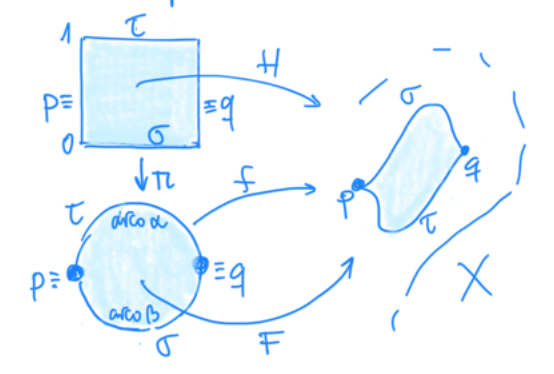
\includegraphics[scale=0.3]{images/def_simple_conx}
    \end{center}
\end{demo}

\begin{ej}
Los conjuntos convexos son simplemente conexos. ¿Los estrellados?
\end{ej}

\section{Esferas \texorpdfstring{$\mathbb{S}^n,\ n \ge 2$}{Sn, n >= 2}}%
\label{sec:esferas_s_n}
\begin{prop}
$\mathbb{S}^n : \{x_1^2 + \ldots + x_{n + 1}^2 = 1\} \subset \mathbb{R}^{n + 1}$ es simplemente conexo ($n \ge 2$).
\end{prop}
\begin{demo}
$\sigma, \tau: \left[ a, b \right] \rightarrow \mathbb{S}^n,\ \sigma\left( a \right) = \tau\left( a \right) = p,\ \sigma\left( b \right) = \tau\left( b \right) = q$.
\[
\exists c, -c \in \mathbb{S}^n\setminus \{p, 1\}\; \land \;\begin{rcases}
   U = \mathbb{S}^n \setminus \{c\} \stackrel{\text{homeo.}}{\approx} \mathbb{R}^n\\
   V = \mathbb{S}^n \setminus \{-c\} \stackrel{\text{homeo.}}{\approx} \mathbb{R}^n
\end{rcases} \text{proyección estéreo.}  
\]
\begin{enumerate}
    \item $\left[ a, b \right] \subset \sigma^{-1}U \cup \sigma^{-1}V \xRightarrow{\text{comp.}} \exists a = t_0 < t_1 < \ldots < t_r = 1: \sigma\left[ t_{i - 1}, t_1 \right] \begin{cases}
        \subset U\\
        \subset V
    \end{cases}$ dónde $\sigma\left[ t_{i - 1}, t_i \right]$ es la traza de $\sigma_i = \sigma|_{\left[ t_{i - 1}, t_i \right]}$.

    \item Si dos consecutivos están en el mismo $U$ ó $V$, eliminamos la juntura común $\Rightarrow$ al atravesar una juntura $t_k$ cambiamos de $U$ a $V$ ó viceversa, en particular, $x_k = \sigma\left( t_k \right) \in U \cap V \approx \mathbb{R}^n \setminus \{\text{punto}\}$, que es conexo por caminos, o bien, nos quedamos sin junturas y $\sigma\left[ a, b \right] \subset U$ ó $V$.

    \item Consideramos los trozos en $V$ (incluido que $\sigma\left[ a, b \right] \subset V$ porque no hay ya junturas)
    \begin{center}
        \includegraphics[scale=0.3]{images/esferas_sn_3} 
    \end{center}
    \begin{itemize}
        \item[(*)]
        \begin{align*}
            \sigma\left( t_{i - 1} \right), \sigma\left( t_i \right) \in U \cap V &\approx \mathbb{R}^n \setminus \{\text{punto}\} \text{ conexo por caminos}\\
            &\Rightarrow \exists \sigma_i^*: \left[ t_{i - 1}, t_i \right] \rightarrow U\cap V \subset V \text{ mismos extremos que } \sigma_i
        .\end{align*}

        \item[(**)] $V \approx \mathbb{R}^n$ convexo $\Rightarrow \exists H_s^i: \sigma_i \simeq \sigma_i^*$ en $V$ con extremos fijos. ¡Ojo! $\boxed{\sigma_i^*: \left[ t_{i - 1}, t_i \right] \rightarrow U}$.
    \end{itemize}

    \item Pegando a trozos homotopías en $\mathbb{S}^n$:
    \[
    \begin{cases}
        \sigma\left[ t_{i_1}, t_i \right] \subset U \Rightarrow H_s^i \equiv \sigma_i = \sigma_i^*: \left[ t_{i - 1}, t_i \right] \rightarrow U \subset \mathbb{S}^n\\
        \sigma\left[ t_{i_1}, t_i \right] \subset V \xRightarrow{3} H_s^i : \sigma_i \simeq \sigma_i^*: \left[ t_{i - 1}, t_i \right] \rightarrow V \subset \mathbb{S}^n
    \end{cases} \Rightarrow \sigma \simeq \sigma^* 
    \]
    Homótopos en $\mathbb{S}^n$ con extremos fijos, pero $\sigma^*\left[ a, b \right] \subset U$.

    \item Igual, $\exists H_s: \tau \simeq \tau^*$ homotopía en $\mathbb{S}^n$ con extremos fijos, pero $\tau^*\left[ a, b \right] \subset U$.
\end{enumerate}
En conclusión: $\sigma^* \simeq \tau^*$ en $U \left( \approx \mathbb{R}^n \right)$ con extremos fijos $\Rightarrow \sigma \simeq \sigma^* \simeq \tau^* \simeq \tau$ con extremos fijos.
\end{demo}
